\documentclass[a4paper,12pt]{article}
\usepackage[english,russian]{babel}
\usepackage{fontspec}
\defaultfontfeatures{Ligatures={TeX},Renderer=Basic}
\setmainfont[Ligatures={TeX,Historic}]{Calibri Light}
\setsansfont{Calibri Light}
\setmonofont{Consolas}

\usepackage{indentfirst}
\frenchspacing

% Для математики
\usepackage{amssymb,amsmath}
\setcounter{MaxMatrixCols}{20}
\parindent=24pt
\parskip=0pt
\tolerance=2000

% Для настройки размера страницы
\usepackage{geometry}
\geometry{
	a4paper,
	total={170mm,257mm},
	left=20mm,
	top=20mm,
}

% Для вставки графики
\usepackage{graphicx}
\usepackage{hyperref}

% Для таблиц
\usepackage{longtable}
\usepackage{multirow}
\usepackage{tabu}
\usepackage{colortbl}
\usepackage{hhline}
\usepackage{tabularx}
\usepackage{booktabs}
\usepackage[table]{xcolor} 

% Создаем команду, чтобы переносить текст на новую строку внутри таблицы
\newcommand{\tcell}[1]{\begin{tabular}{@{}c@{}}#1\end{tabular}}
\newcommand{\ltcell}[1]{\begin{tabular}{@{}l@{}}#1\end{tabular}}

% Пакет для списков
\usepackage[ampersand]{easylist}

% Для контура вокруг текста
\usepackage[outline]{contour}

% Пакеты от tikz
\usepackage{tikz}
\usepackage{graphics}
\usepackage{pgfplots}
\usepackage{pgfplotstable}
\usepackage{xcolor}
\usetikzlibrary{calc}
\usetikzlibrary{through}
\usetikzlibrary{intersections}
\usetikzlibrary{patterns}
\usetikzlibrary{scopes}
\usetikzlibrary{decorations.pathreplacing}
\usetikzlibrary{arrows.meta}

% Для цветных таблиц
\usepackage{multicol}
\usepackage{tcolorbox}
\tcbuselibrary{skins}
\tcbuselibrary{breakable}
\tcbuselibrary{minted}
\usemintedstyle{vs}

% Для подсветки кода
\usepackage{minted}

% Задаем цвет номеров строк подсветки кода
\renewcommand{\theFancyVerbLine}{\sffamily\textcolor[rgb]{1, 1, 1}{\fontsize{4}{4}\selectfont\arabic{FancyVerbLine}}}

% Определяем новую команду для красивой вставки кода в рамочке и с прочими прелестями
\newcommand{\mycodeinput}[3]{
\begin{tcolorbox}[
	colback=black!5!white,
	colframe=black!30!white,
	boxrule=0.5pt, 
	listing only,
	left=-0.5mm,
	leftrule=3.3mm,
	arc=2mm, outer arc=2mm,
	top=0pt,
	bottom=0pt,
	enhanced jigsaw,
	breakable,
	title={#3},
	coltitle=black, 
	fonttitle=\bfseries\ttfamily,
	break at=-\baselineskip/0pt/\textheight, % Магия для работы multicols
	attach boxed title to top center={yshift=-1mm,yshifttext=-1mm},
	boxed title style={
		enhanced,
		nobeforeafter,
		tcbox raise base,
		boxrule=0.4pt,
		top=0.5mm,
		bottom=0.5mm,
		right=0mm,
		left=4mm,
		arc=1pt,
		boxsep=2pt,
		before upper={\vphantom{dlg}},
		colframe=black!30!white,
		colback=black!10!white,
		overlay={
			\begin{tcbclipinterior}
			\fill[black!30!white]
				(frame.south west)
					rectangle node[text=white,font=\sffamily\bfseries\scriptsize,rotate=90] {FILE} 
				([xshift=4mm]frame.north west);
			\end{tcbclipinterior}
		}
	},
]
\inputminted[
	breaklines,
	breakanywhere=true,
	autogobble,
	linenos,
	numbersep=1mm,
	mathescape, 
	fontsize=\fontsize{8}{8}\selectfont, 
	tabsize=4
]{#1}{#2}
\end{tcolorbox}
}

% Определяем новую команду для вставки кода прямо в тексте
\newtcbox{\inlinecodetable}{on line,
arc=2pt,colback=gray!10!white,colframe=gray!50!black,
before upper={\rule[-3pt]{0pt}{10pt}},boxrule=0.5pt,
boxsep=0pt,left=2pt,right=2pt,top=2pt,bottom=0pt}
\newcommand{\mycodeinline}[2]{\inlinecodetable{\mintinline{#1}{#2}}}

% Определяем новую команду для создания титульного листа
\newcommand{\mytitlepage}[9]{
\begin{center}
\hfill \break
\Large{Министерство образования и науки Российской Федерации}\\
\hfill \break
\large{Федеральное государственное бюджетное образовательное учреждение высшего образования}\\ 
\normalsize{\textbf{«НОВОСИБИРСКИЙ ГОСУДАРСТВЕННЫЙ ТЕХНИЧЕСКИЙ УНИВЕРСИТЕТ»}}\\
\hfill \break

\includegraphics{nstu_logo.eps} \\
\hfill \break
\large{Кафедра #1}\\
\hfill \break
\large{Лабораторная работа №#2\\по дисциплине <<#3>>}\\
\hfill \break
\hfill \break
\Large{\textbf{#4}}\\
\hfill \break
\hfill \break 
\normalsize{\begin{tabular}{cllp{1.5cm}p{1.5cm}}
\multirow{5}{*}[0.75cm]{
\includegraphics[scale=0.5]{fami_logo.eps}}
& \textbf{Факультет:} & ПМИ & & \\[1.25ex]
& \textbf{Группа:} & #5 & & \\[1.25ex]
& \textbf{Студенты:} & #6 & & \\[1.25ex]
& \textbf{Вариант:} & #7 & & \\[1.25ex]
& \textbf{Преподаватель:} & #8 & & \\[1.25ex]
\end{tabular}} \\
\hfill \break
\hfill \break
\hfill \break
\hfill \break
\hfill \break
\large{Новосибирск\\#9}
\end{center}
\thispagestyle{empty}
\newpage 
\setcounter{page}{1}
}

\begin{document}

\pgfplotstableset{
	begin table={\rowcolors{2}{gray!25}{white}\begin{tabular}},
	end table=\end{tabular},
}

\newcommand{\typesetfirsttable}[1]{
\noindent\begin{center}\pgfplotstabletypeset[
	skip first n=1,
	columns/10^i/.style={column name={$\varepsilon = 10^i$},},
	columns/iter/.style={column name={\scriptsize Итераций},},
	columns/fCount/.style={column name={\scriptsize Вычислений $f$},},
	columns/answer/.style={string type, column name={\scriptsize Ответ},},
	columns/restriction_value/.style={column name={$G(\mathbf{x})$},},
	columns/grad.norm()/.style={column name={$||\nabla f(x, y)||_{L_2}$}, column type/.add={}{|},},
	every head row/.style={before row=\hline,after row=\hline\hline}, 
	every last row/.style={after row=\hline},
	column type/.add={|}{},
	col sep=tab,
]{#1.txt}
\end{center}
}

\newcommand{\typesetsecondtable}[1]{
\noindent\begin{center}\pgfplotstabletypeset[
	skip first n=1,
	columns/n/.style={column name={$n$},},
	columns/iter/.style={column name={\scriptsize Итераций},},
	columns/fCount/.style={column name={\scriptsize Вычислений $f$},},
	columns/answer/.style={string type, column name={\scriptsize Ответ},},
	columns/restriction_value/.style={column name={$G(\mathbf{x})$},},
	columns/grad.norm()/.style={column name={$||\nabla f(x, y)||_{L_2}$}, column type/.add={}{|},},
	every head row/.style={before row=\hline,after row=\hline\hline}, 
	every last row/.style={after row=\hline},
	column type/.add={|}{},
	col sep=tab,
]{#1.txt}
\end{center}
}

\newcommand{\typesetfourgraphs}[1]{
\noindent\begin{tikzpicture}
\begin{semilogyaxis}[xlabel=Начальное значение штрафа,ylabel=\tcell{\scriptsize Вычислений\\\scriptsize функции},width=\textwidth, height=4cm]
\addplot[blue, no markers] table [skip first n=1, y=fCount, x=startPenaltyCoef]{table_start_#1.txt};
\end{semilogyaxis}
\end{tikzpicture}

\noindent\begin{tikzpicture}
\begin{axis}[xlabel=Начальное значение штрафа,ylabel=Итераций,width=\textwidth, height=4cm]
\addplot[red, no markers] table [skip first n=1, y=iter, x=startPenaltyCoef]{table_start_#1.txt};
\end{axis}
\end{tikzpicture}

\noindent\begin{tikzpicture}
\begin{semilogyaxis}[xlabel=Коэффициент увеличения штрафа,ylabel=\tcell{\scriptsize Вычислений\\\scriptsize функции},width=\textwidth, height=4cm]
\addplot[blue, no markers] table [skip first n=1, y=fCount, x=penaltyExponent]{table_exp_#1.txt};
\end{semilogyaxis}
\end{tikzpicture}

\noindent\begin{tikzpicture}
\begin{axis}[xlabel=Коэффициент увеличения штрафа,ylabel=Итераций,width=\textwidth, height=4cm]
\addplot[red, no markers] table [skip first n=1, y=iter, x=penaltyExponent]{table_exp_#1.txt};
\end{axis}
\end{tikzpicture}
}

%------------------------------------------------------------------------------
%------------------------------------------------------------------------------
%------------------------------------------------------------------------------

\mytitlepage{прикладной математики}{3}{Методы оптимизации}{Метод штрафных функций}{ПМ-63}{
\ltcell{Шепрут И.И.\\Крашенинник Н.А.\\Пешкичева А.А.}}{4}{Чимитова Е.В.}{2019}

\section{Цель работы}

Ознакомиться с методами штрафных функций при решении задач нелинейного программирования. Изучить типы штраф¬ных и барьерных функций, их особенности, способы и области применения, влияние штрафных функций на сходимость алгоритмов, зависимость точности решения задачи нелинейного программирования от величины коэффициента штрафа.

\section{Задание}

\noindent\begin{easylist}
\ListProperties(Hang1=true, Margin2=12pt, Style1**=$\bullet$ , Hide2=1, Hide1=1)
& Применяя методы поиска минимума 0-го порядка, реализовать программу для решения задачи нелинейного программирования с использованием метода штрафных функций/барьерных функций.
& Исследовать сходимость метода штрафных функций/барьерных функций в зависимости от:
&& выбора штрафных функций,
&& начальной величины коэффициента штрафа,
&& стратегии изменения коэффициента штрафа,
&& начальной точки,
&& задаваемой точности.
& Сформулировать выводы.
\end{easylist}

\noindent\textbf{Вариант:}

\noindent4. $f(x, y) = 2(x-y)^2+14(y-3)^2 \rightarrow min$

при ограничении:

a) $y-x \geqslant 0.2$

б) $x = -y$

\section{Исследования}

Во всех исследованиях, если не указано иное: $\varepsilon = 10^{-7}$; коэффициент увеличения штрафа: $2$; начальный коэффициент штрафа: $1$; начальное приближение: $(-1, 0)^T$; стратегия изменения штрафа: домножать текущий штраф на коэффициент увеличения штрафа.

\subsection{$y-x-0.2 \geqslant 0$}

Функция штрафа для этого случая:

$$ G = \left\{\begin{aligned}
&0, && y - x-0.2 \geqslant 0, \\
&-(y-x-0.2), && \text{иначе}
\end{aligned}\right. $$

Таблица исследования в зависимости от требуемой стартовой точности:

\typesetfirsttable{table_eps_1}

Зависимость числа вычислений функции от начальной точки. Чем темнее пиксель, тем больше требуется вычилений функции. начиная с этой точки; чем светлее, тем меньше. Границы на изображении: $[-3, 3]\times[-3, 3]$. Сверху слева показана информация о числе вычислений функции для сходимости метода из этой точки.

\noindent\begin{center}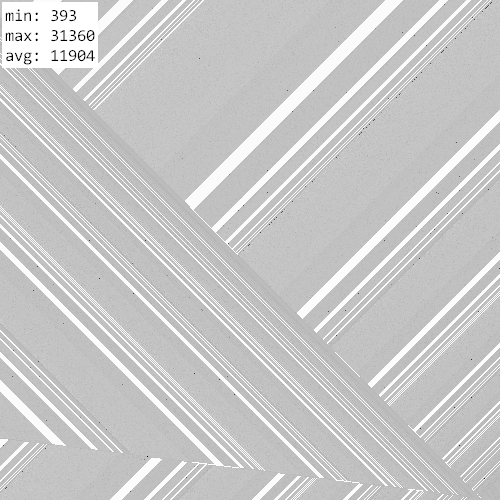
\includegraphics[width=.5\textwidth]{1.png}\end{center}

Зависимость числа итераций и вычислений функции в зависимости от начального значения штрафа и коэффициента увеличения штрафа:

\typesetfourgraphs{1}

\subsubsection{Исследования стратегии изменения штрафа}

$$ g = 100(x-y+0.2) $$

Для изменения функции штрафа была выбрана следующая функция. Будет исследовано как она влияет на процесс в зависимости от $n$:

$$ G = \left(\frac{g+|g|}{2}\right)^{2n} $$

\typesetsecondtable{table_fine_g}

\subsection{$x=-y$}

Функция штрафа для этого случая:

$$G = |x+y|$$

Таблица исследования в зависимости от требуемой стартовой точности:

\typesetfirsttable{table_eps_2}

Зависимость числа вычислений функции от начальной точки. Чем темнее пиксель, тем больше требуется вычилений функции. начиная с этой точки; чем светлее, тем меньше. Границы на изображении: $[-3, 3]\times[-3, 3]$. Сверху слева показана информация о числе вычислений функции для сходимости метода из этой точки.

\noindent\begin{center}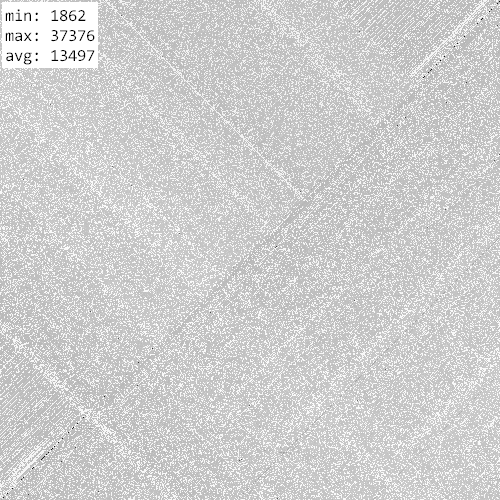
\includegraphics[width=.5\textwidth]{2.png}\end{center}

Зависимость числа итераций и вычислений функции в зависимости от начального значения штрафа и коэффициента увеличения штрафа:

\typesetfourgraphs{2}

\subsection{Барьерная функция}

Коэффициент увеличения штрафа: $0.5$ (чтобы штраф уменьшался).

$$ g = 100(x-y+0.2) $$

Функция штрафа для этого случая:

$$ G = \left\{\begin{aligned}
&-\ln(-g), && g < 0, \\
&\infty, && \text{иначе}
\end{aligned}\right. $$

Таблица исследования в зависимости от требуемой стартовой точности:

\typesetfirsttable{table_eps_3}

Зависимость числа итераций и вычислений функции в зависимости от начального значения штрафа и коэффициента увеличения штрафа:

\typesetfourgraphs{3}

\section{Выводы}

\noindent\begin{easylist}
\ListProperties(Start1=1, Hang1=true, Margin2=12pt, Style1**=, Style2**=$\bullet$ , Hide2=2, Hide1=0)
& \textit{Об объеме вычислений в зависимости от требуемой точности:}
&& Для простых штрафных функий требуемая точность практически не влияет на число вычислений.
&& Для барьерных функций требуемая точность значительно влияет на число итераций. Чем больше требуется точность, тем больше итераций.
& \textit{Об объеме вычислений в зависимости от начального приближения:} по обоим изображениям видно, что нет никакой закономерности. Хотя, возможно, потому что исследуется на квадратичной функции.
& \textit{Об объеме вычислений в зависимости от начальной величины штрафа и коэффициента изменения штрафа:} делается на основе построенных графиков
&& Для штрафных функций оптимальное начальное значение --- $10$, коэффициент увеличения штрафа --- $10$.
&& Для барьерных функций оптимальное начальное значение --- $0.1$, коэффициент увеличения штрафа --- $0.1$.
& \textit{Об объеме вычислений в зависимости от выбора штарфных функций:} функция $ G = \left(\frac{g+|g|}{2}\right)^{2n} $ практически никак не повлияла на сходимость и объем вычислений.
\end{easylist}

\section{Код}

\subsection{Заголовочные файлы}

\mycodeinput{c++}{../methods3.h}{methods3.h}
\mycodeinput{c++}{../visualize.h}{visualize.h}

\subsection{Файлы исходного кода}

\mycodeinput{c++}{../test.cpp}{make\_tables.cpp}
\mycodeinput{c++}{../methods3.cpp}{methods3.cpp}
\mycodeinput{c++}{../visualize.cpp}{visualize.cpp}

\end{document}